\appendix{System Configuration (ImProver2)}
\label{app:config_improver2}



\subsection{Training}


\begin{figure*}
\centering
\begin{minipage}{0.32\linewidth}
    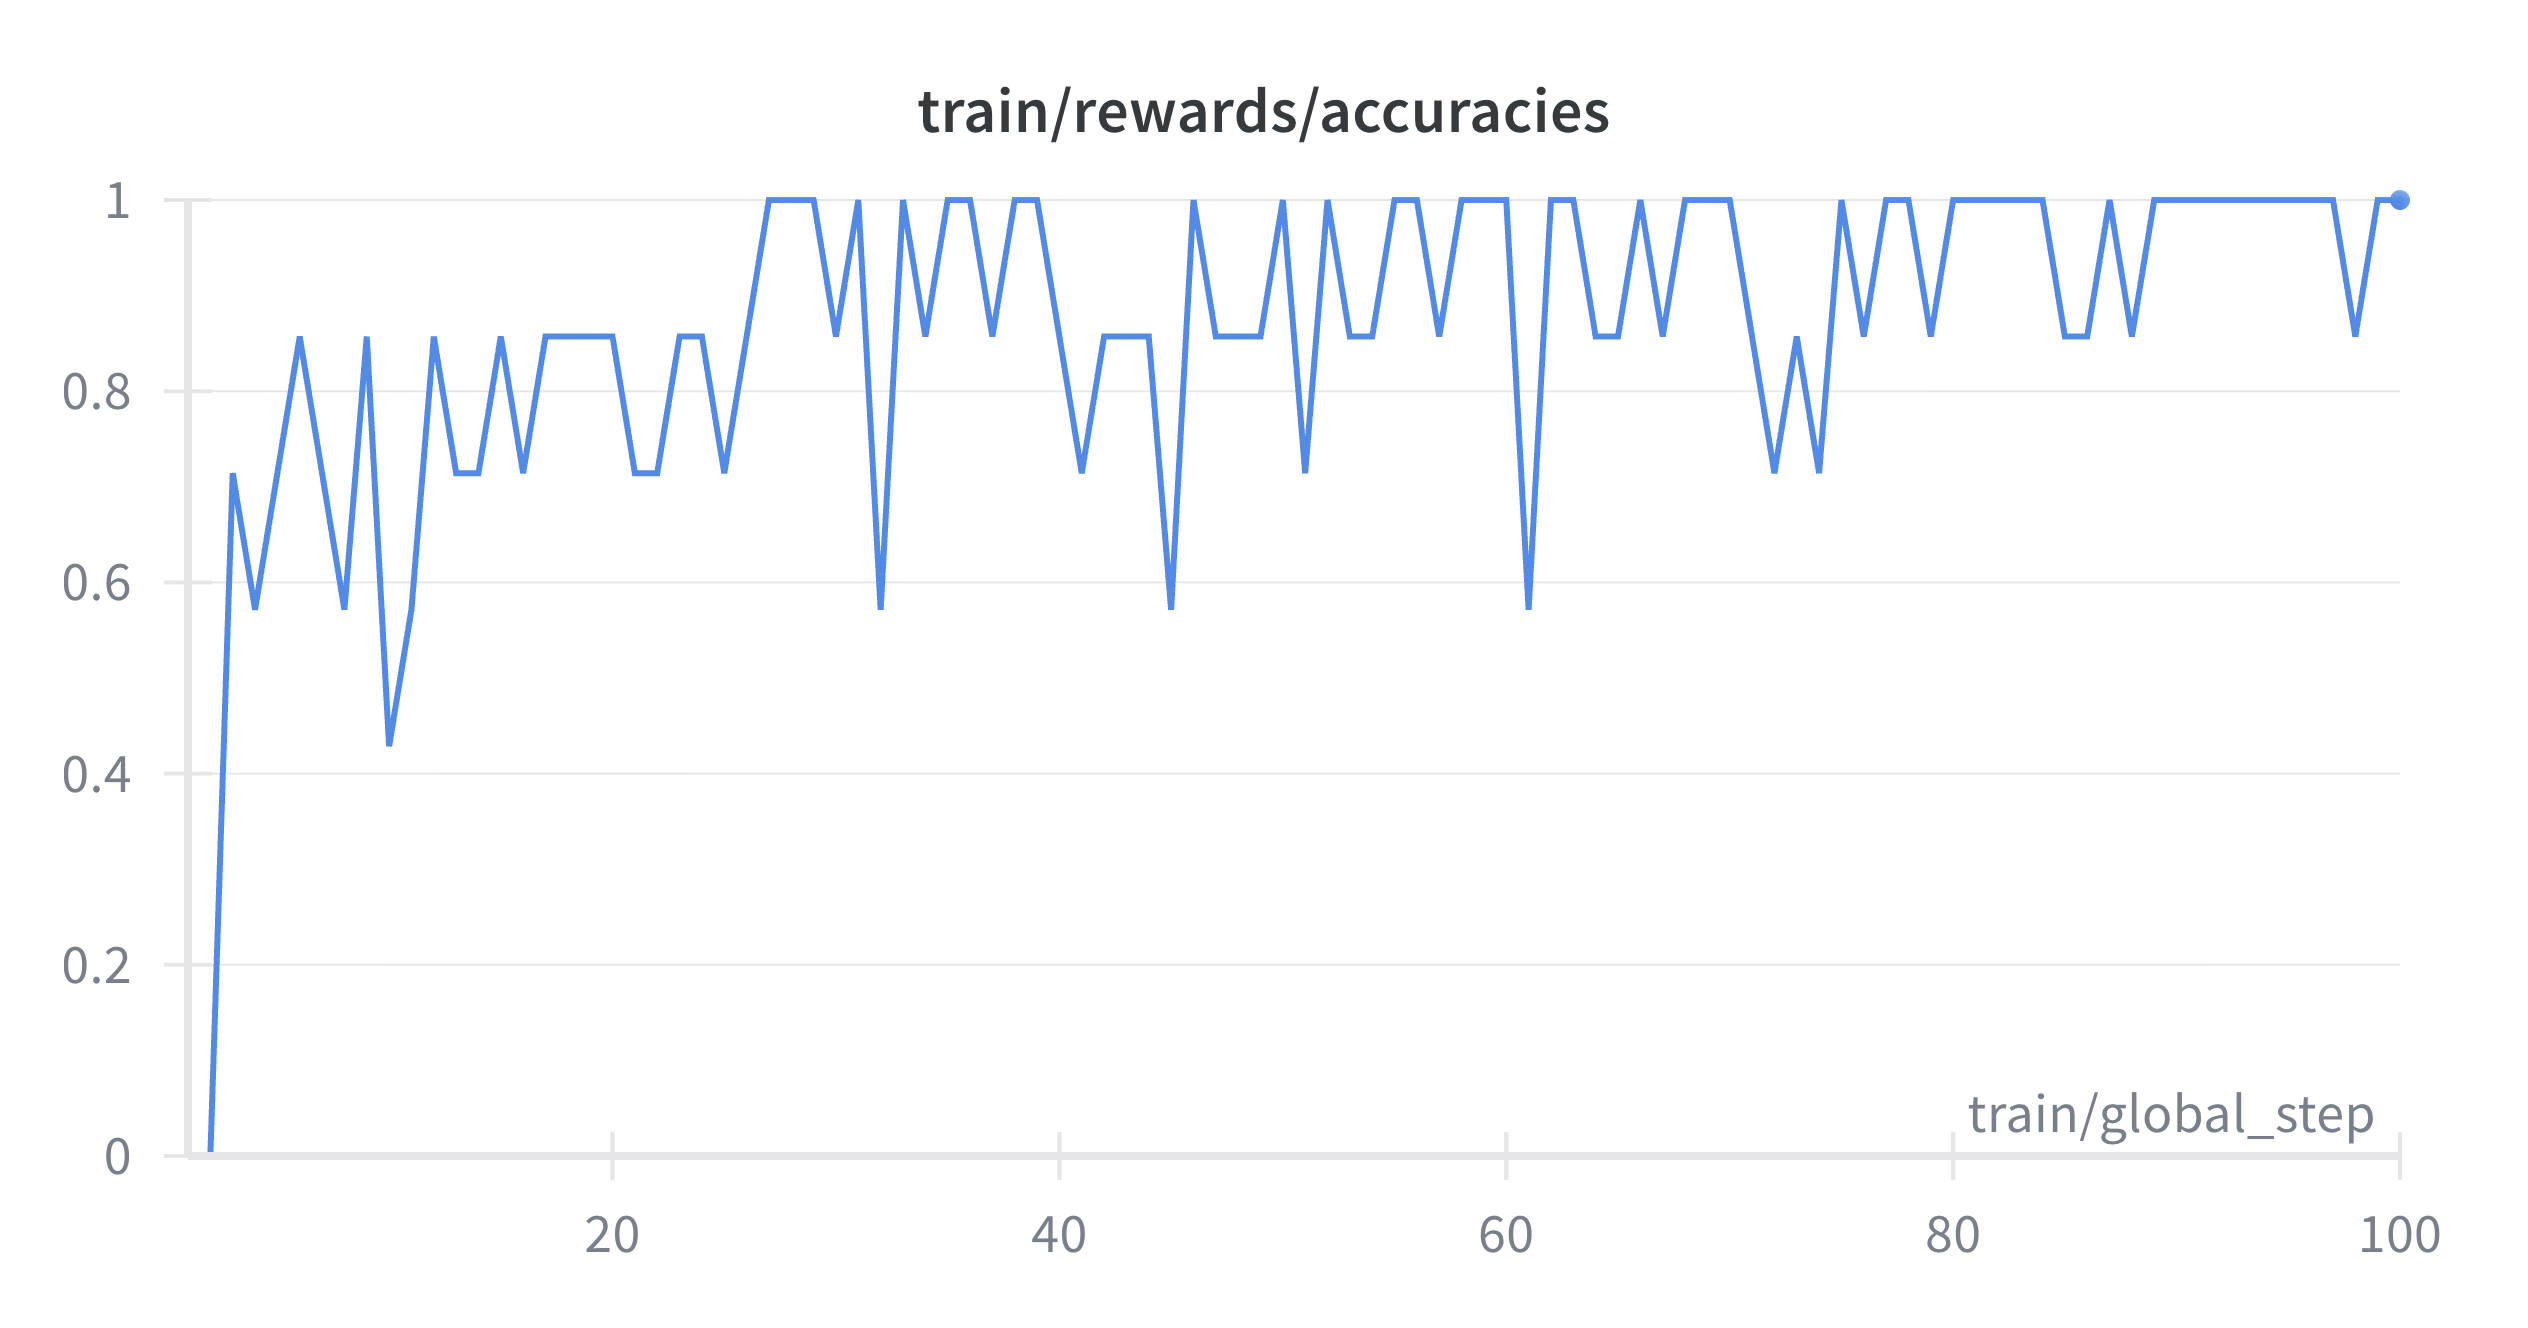
\includegraphics[width=\textwidth]{figures/Dependency/IRPO Dependency Iter 3 Acc.png}
    \scriptsize Training accuracy over time on iteration 3 of the dependency metric.
\end{minipage}
\hfill
\begin{minipage}{0.32\linewidth}
    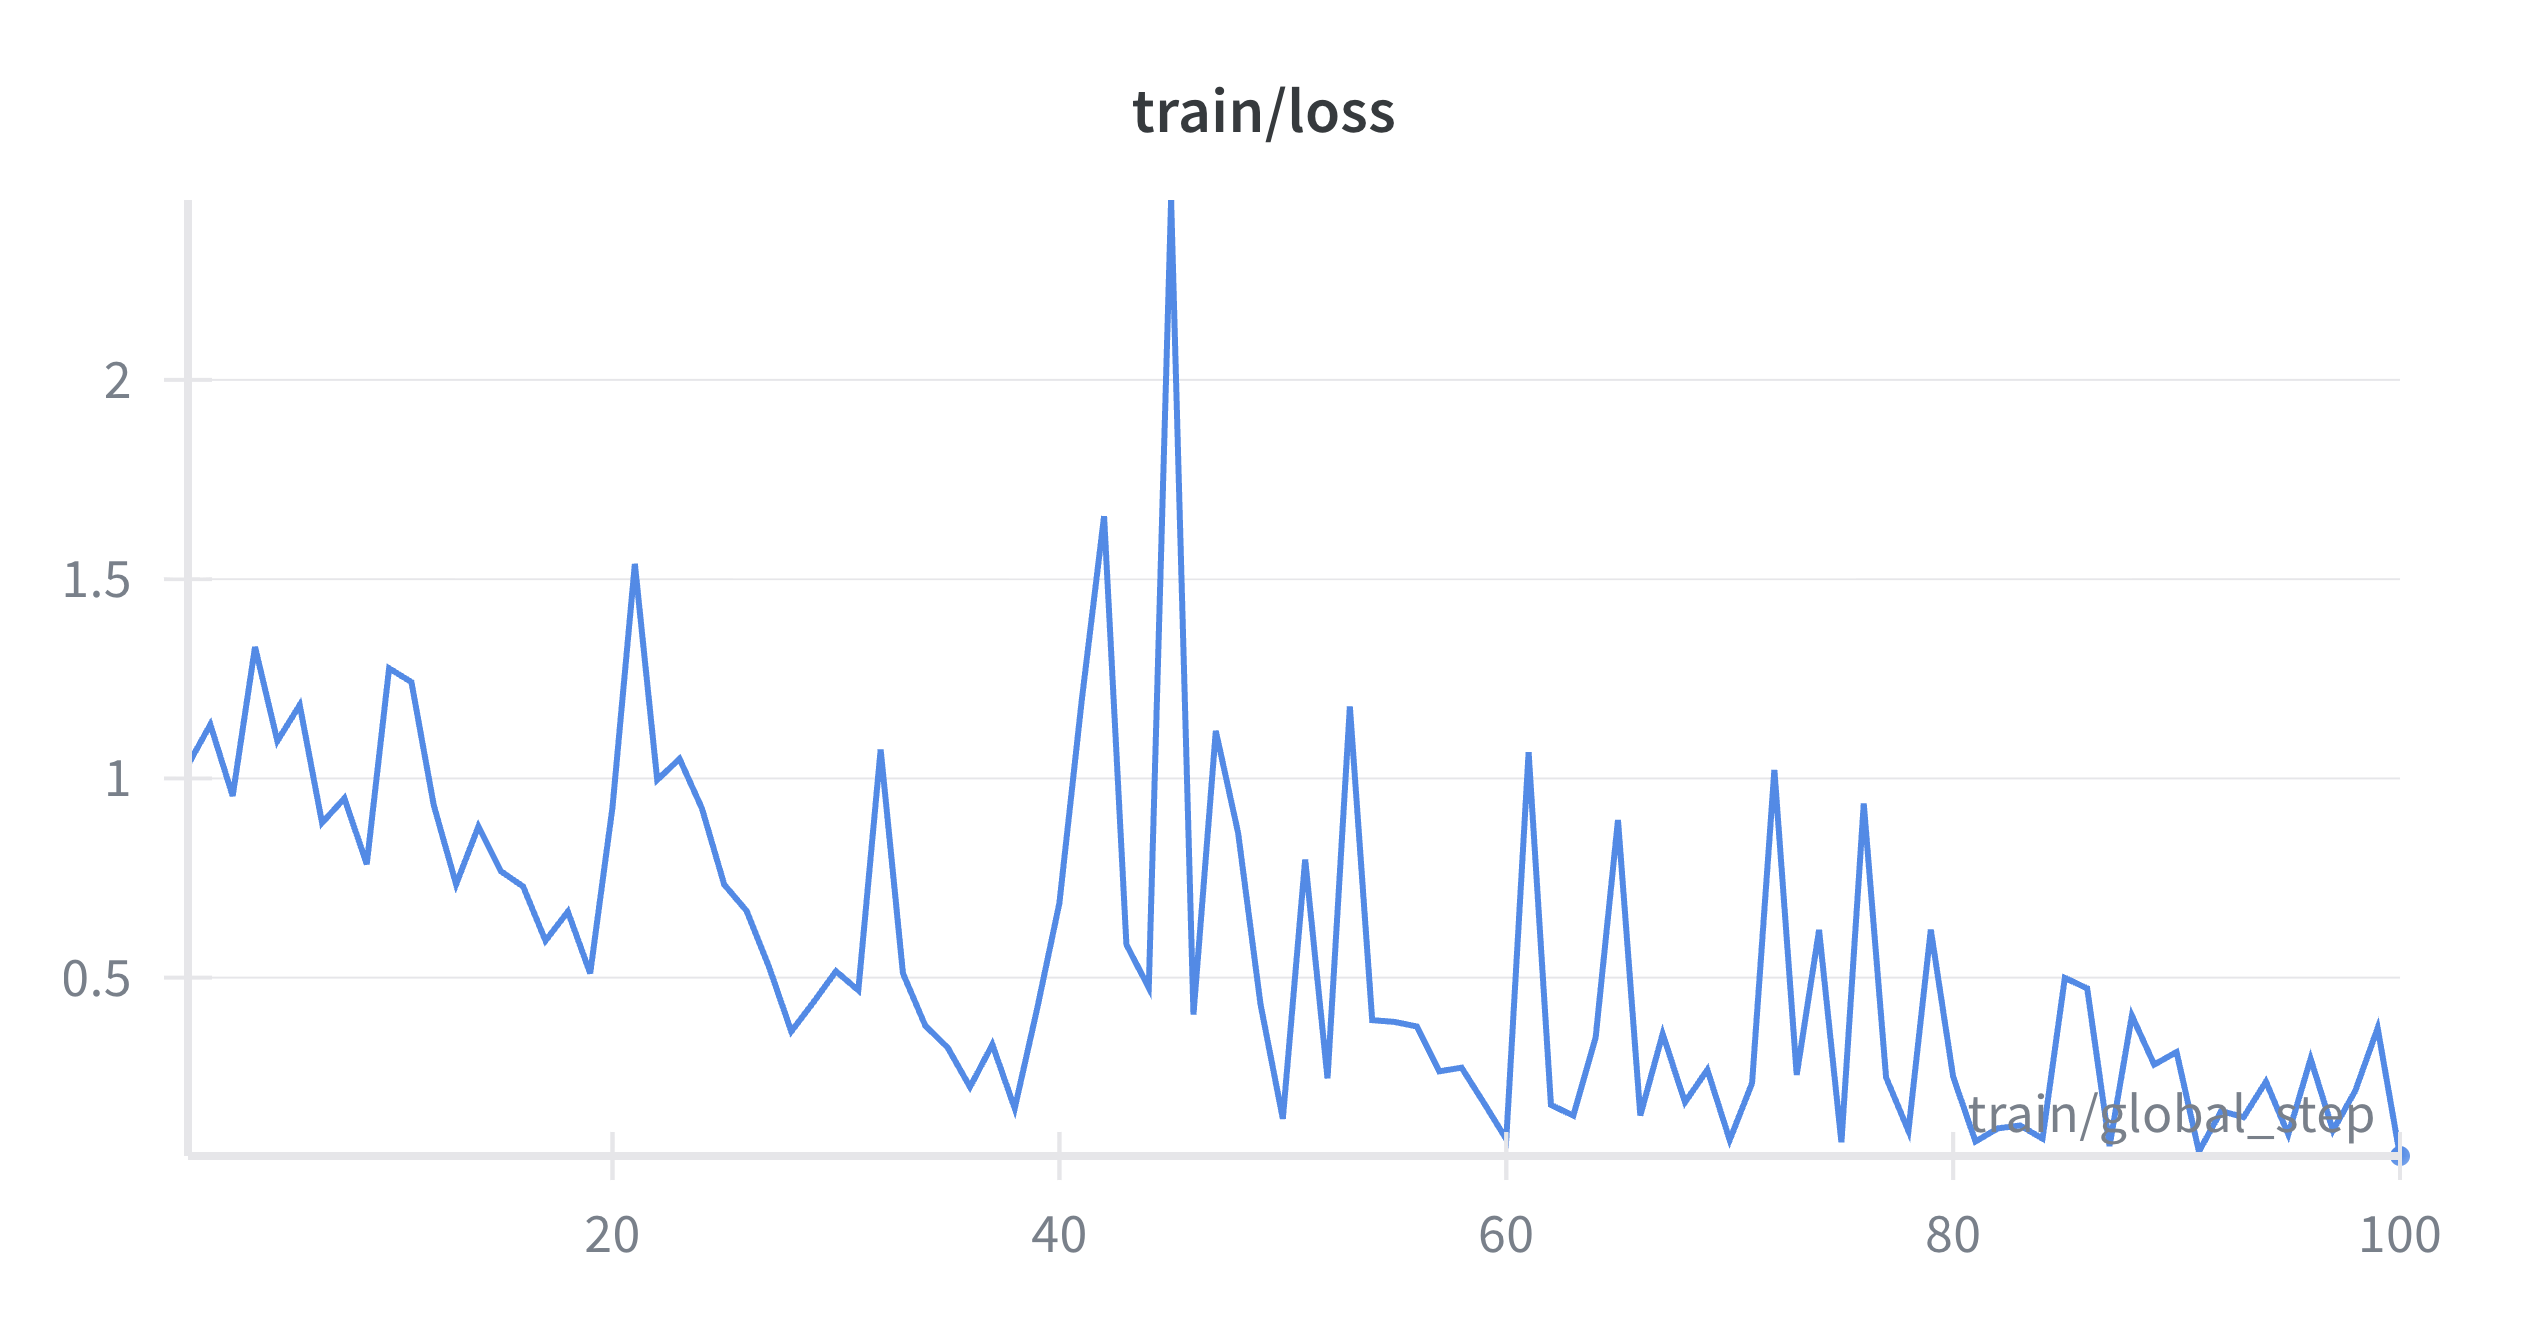
\includegraphics[width=\textwidth]{figures/Dependency/IRPO Dependency Iter 3 Loss.png}
    \scriptsize Training loss over time on iteration 3 of the dependency metric.
\end{minipage}
\hfill
\begin{minipage}{0.32\linewidth}
    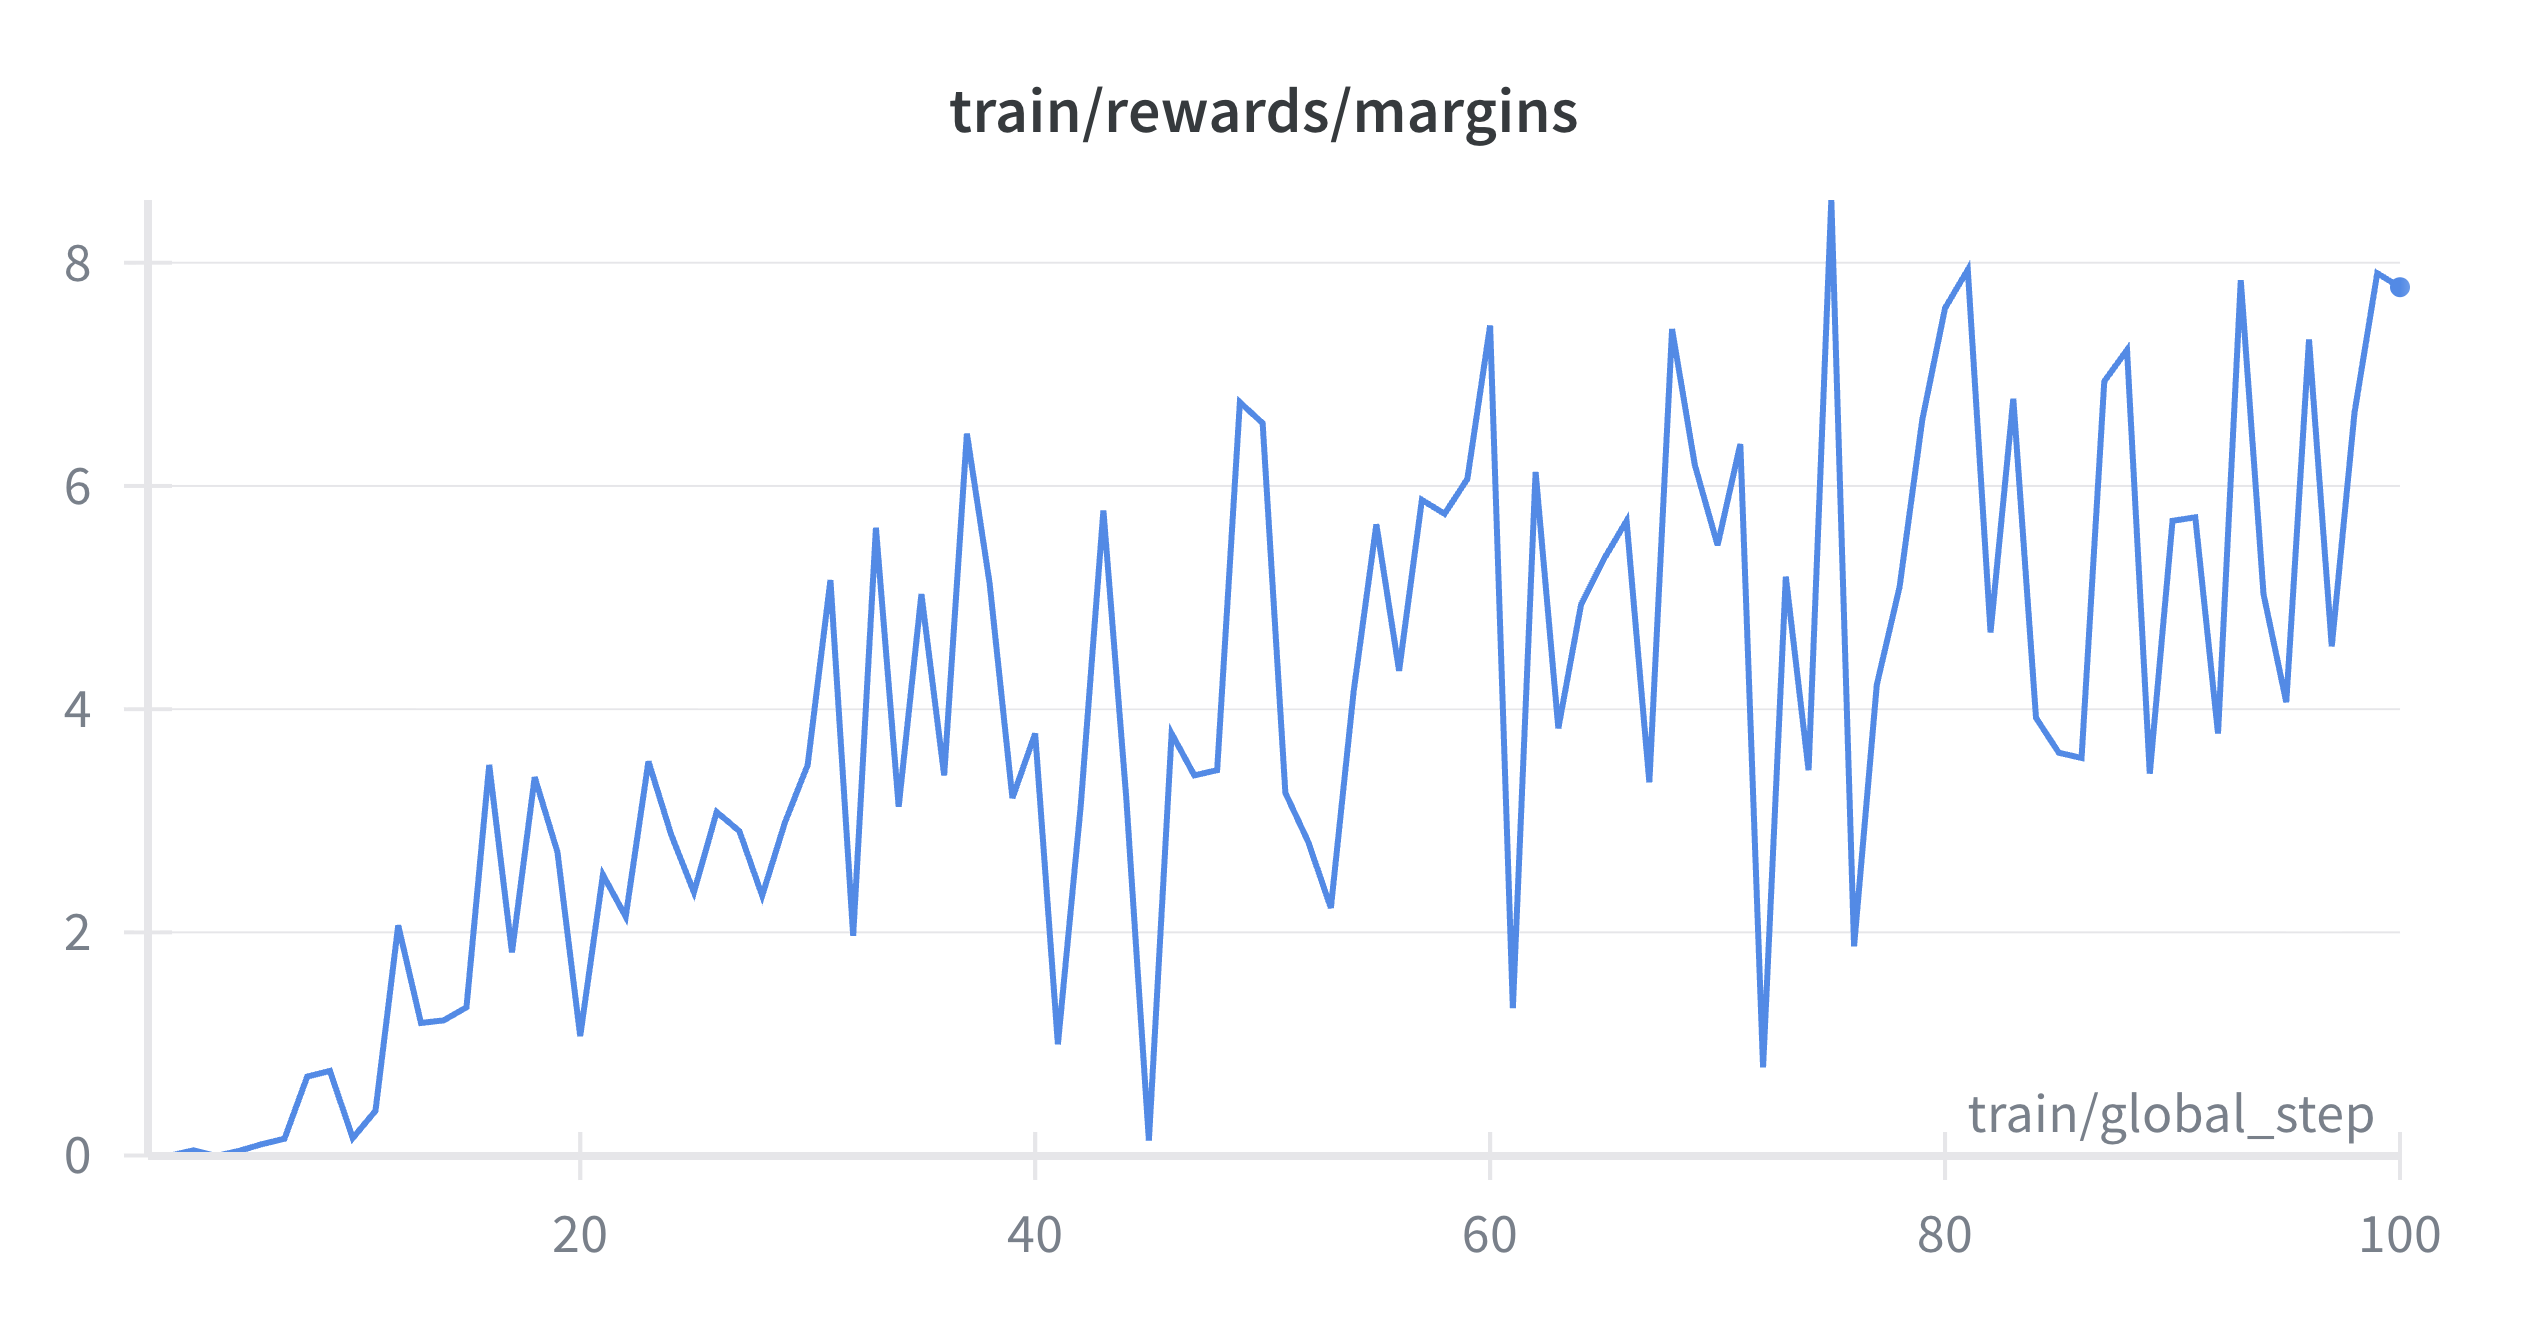
\includegraphics[width=\textwidth]{figures/Dependency/IRPO Dependency Iter 3 Margin.png}
    \scriptsize Average margin over time during training on iteration 3 of the dependency metric.
\end{minipage}
\caption{Training statistics during iteration 3 of the dependency metric. Model shows stable performance despite overall regression on this iteration. }

\end{figure*}



\subsection{System Prompts}

During generation, \ImProver \ is prompted by combining the following prompts: depending on the metric, we take one of the \textbf{length}, \textbf{modularity}, or \textbf{dependency} prompts, and append the \textbf{annotation}, \textbf{context}, and \textbf{examples} prompts along with the relevant neurosymbolic augmentation in the correct locations. 

\paragraph{Length:}

\tiny\texttt{You are an expert Lean4 theorem rewriting assistant. Shorten the current Lean4 theorem (wrapped in <CURRENT>...</CURRENT>) to be as short as possible in length - measured in the number of tactics in the proof - while also ensuring that the output is still a correct proof of the theorem. Be sure to output your final response as a Lean4 theorem wrapped in <IMPROVED>...</IMPROVED> tags, as shown in the example. Namely, only return the statement and proof of the current theorem in Lean4 code, wrapped in <IMPROVED>...</IMPROVED> tags. Do not include any other text or comments.}

\paragraph{Modularity:}

\tiny\texttt{You are an expert Lean4 theorem rewriting assistant. Given a Lean4 theorem enclosed in <CURRENT>...</CURRENT> tags, rewrite the theorem to be as modular and declarative as possible. Modularity is defined by the number of independent, meaningful subproofs, measured by the occurrence of tactics that spawn new goals (such as 'have' statements, case splits, automation tactics, or 'calc' blocks) -- with the caveat that these subproofs must be nontrivial and contribute to the overall proof structure. That means any sort of duplicate, unused, or trivial spawned goals will be ignored and/or penalized; this includes trivial modifications to spawned goals such as changing binders into forall statements. etc. Your objective is to maximize the number of these useful, nontrivial, and interesting spawned subproofs, while ensuring that the theorem remains correct and is clearly structured and readable. Optimize and rewrite the proof structure based on genuine sub-arguments, not superficial goal spawning. Validate that the revised theorem remains correct and that improvements in modularity are nontrivial and significant. In your output, only provide the improved statement and proof, wrapped in <IMPROVED>...</IMPROVED> tags, with no additional text or comments. Under no circumstances should you create artificial or superficial modularity in order to optimize for or maximize a reward metric; prioritize exclusively genuine mathematical quality and proof clarity over any gamified optimization.}


\paragraph{Dependency:}

\tiny\texttt{You are an expert Lean4 theorem rewriting assistant. Rewrite the current Lean4 theorem (wrapped in <CURRENT>...</CURRENT>) to be as independent of external theorems and lemmas as possible. Namely, you aim to rewrite the proof to minimize the number of external dependencies - while also ensuring that the output is still a correct proof of the theorem. Be sure to output your final response as a Lean4 theorem wrapped in <IMPROVED>...</IMPROVED> tags, as shown in the example. Namely, only return the statement and proof of the current theorem in Lean4 code, wrapped in <IMPROVED>...</IMPROVED> tags. Do not include any other text or comments.}


\paragraph{Annotation:}

\tiny\texttt{A version of the current theorem with the goal states annotated has also been provided for reference (wrapped in <ANNOTATED>...</ANNOTATED>). Namely, the goal states have been interleaved between tactics as comments to help you better understand the proof and ensure the correctness of your response. Do not include such state comments in your final response.}


\paragraph{Context:}

\tiny\texttt{The proof context, with relevant definitions and theorems, has additionally been provided to help you better understand the proof and ensure the correctness of your response. It is wrapped in <CONTEXT>...</CONTEXT>, with each item wrapped in <ITEM>...</ITEM>.}



\paragraph{Examples:}

\tiny\texttt{Here are some examples of such optimization, as wrapped in <EXAMPLES>...</EXAMPLES>. Note that these examples are for illustrative purposes only and should not be copied directly. Instead, use them to understand the kind of optimization expected and apply similar techniques to the current theorem, using these positive examples as an intuition and guidance on what kinds of optimizations you may do on your current target theorems. Additionally, you will also be provided with a negative example which will be marked as such. Use it to understand common pitfalls and avoid them in your response. Use both the positive and negative examples to guide your optimization of the current theorem.}

\subsection{Autoinformalization}
\label{app:informal}

\normalsize During the generation round at iteration $t=0$, we create informal statements of each theorem for use in neurosymbolic augmentation. This is carried out by prompting the base model $G_0$ with the following:

\tiny\texttt{You are an expert informalizer of formal mathematics to natural language. Namely, given a formal theorem and proof in Lean4,
you will generate an informalized statement of this same theorem in natural language, as well as (2) an informalized, natural language version of the same formal proof
that is aligned with the informal statement. Namely, when informalizing the proof, you should convert each tactic of the formal proof into a natural language step in the informal proof, and thereby, your informal proof should be written as a sequence of steps. Consider the following example:}

\textit{(examples omitted)}

\tiny\texttt{Now, with these examples in mind, it is now your turn to informalize the following formal statement and proof, which is wrapped in <FORMAL>...</FORMAL> tags.}

\tiny\texttt{You may think and reason as much as you want, but ensure that your final answer for (1): the informal statement is wrapped in <STATEMENT>...</STATEMENT> tags, and (2): the informal proof is wrapped in <PROOF>...</PROOF> tags.
Your final answer should have both a <STATEMENT>...</STATEMENT> tag and a <PROOF>...</PROOF> tag, and if there is no formal proof provided in the input, you may simply output <PROOF></PROOF> for the proof after informalizing the statement (i.e. if you are given a theorem without a proof, or a definition/class/etc.).
Input:
<FORMAL>}

\textit{(formal statement of proof is placed here)}

\tiny\texttt{</FORMAL>}

\normalsize The final informal statements are then parsed out for use in neurosymbolic augmentation. 



\subsection{Hyperparameter Grid Search}

\begin{figure}[t]
\centering
\captionsetup{skip=4pt}

\begin{minipage}[t]{\linewidth}
  \centering
  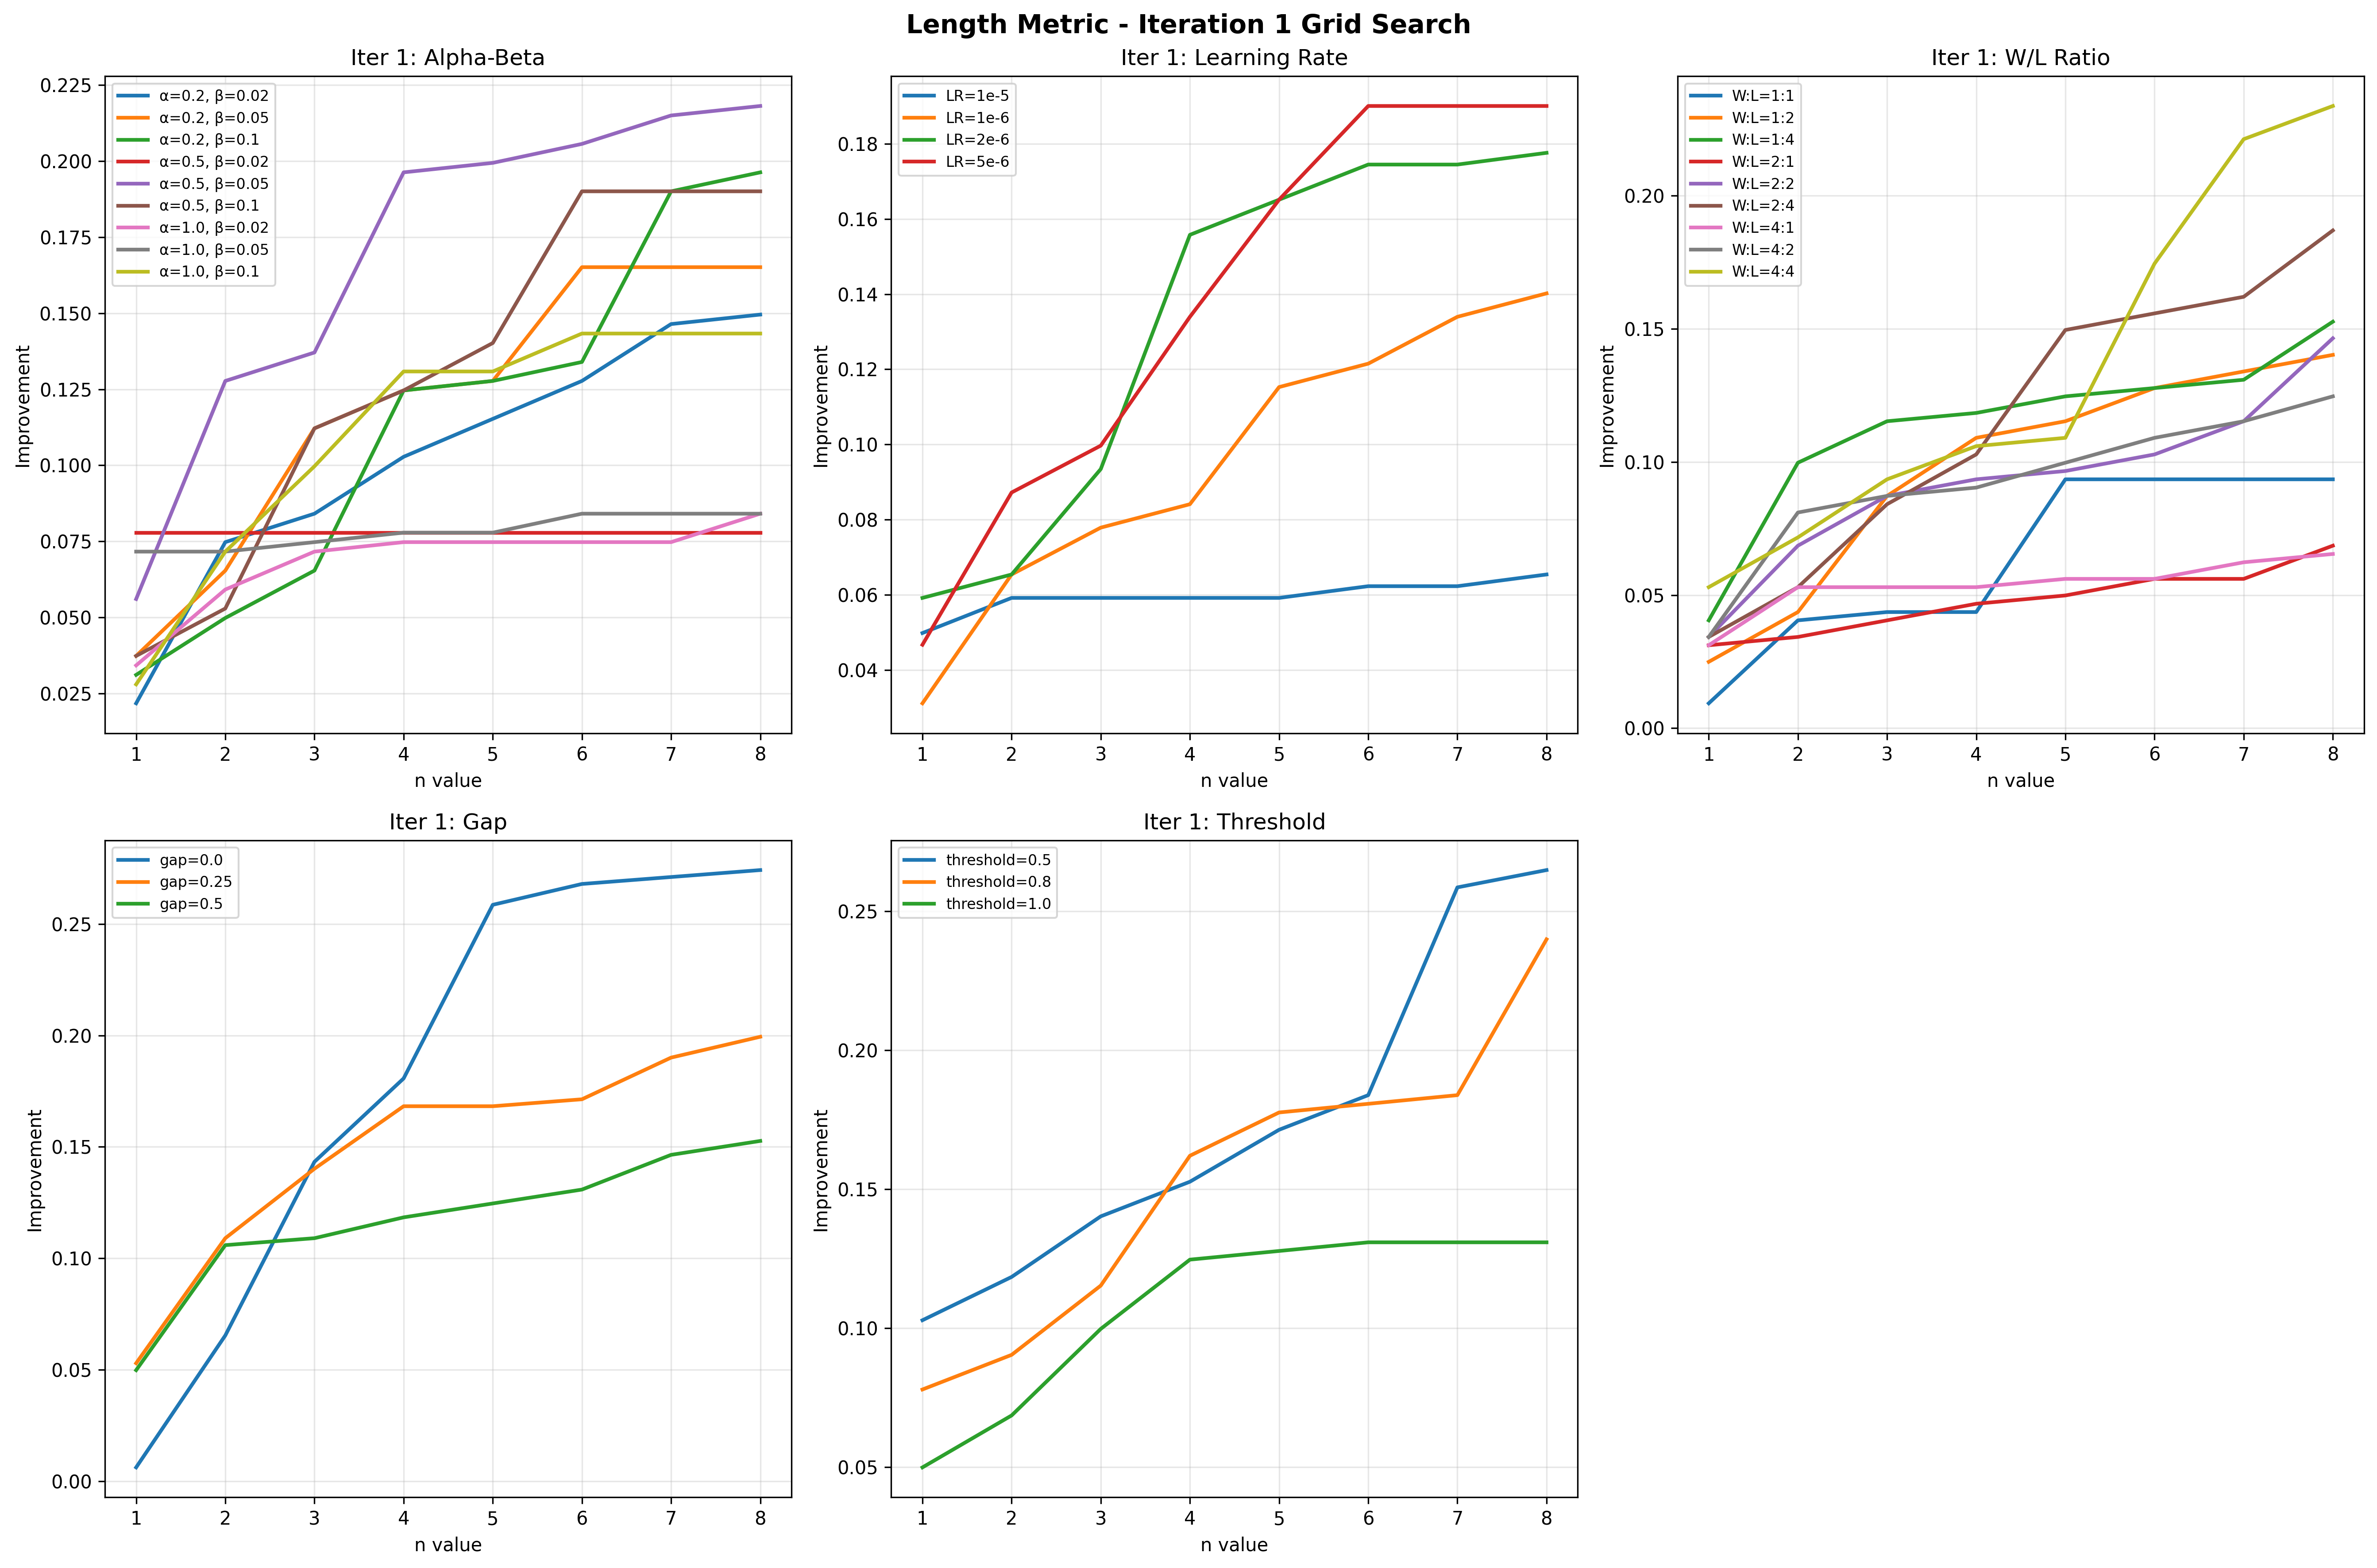
\includegraphics[width=0.65\linewidth]{figures/Length/length_iter_1_gridsearch_all.png}
  % \caption{Iteration 1.}
\end{minipage}

% \vspace{-6pt}

\begin{minipage}[t]{\linewidth}
  \centering
  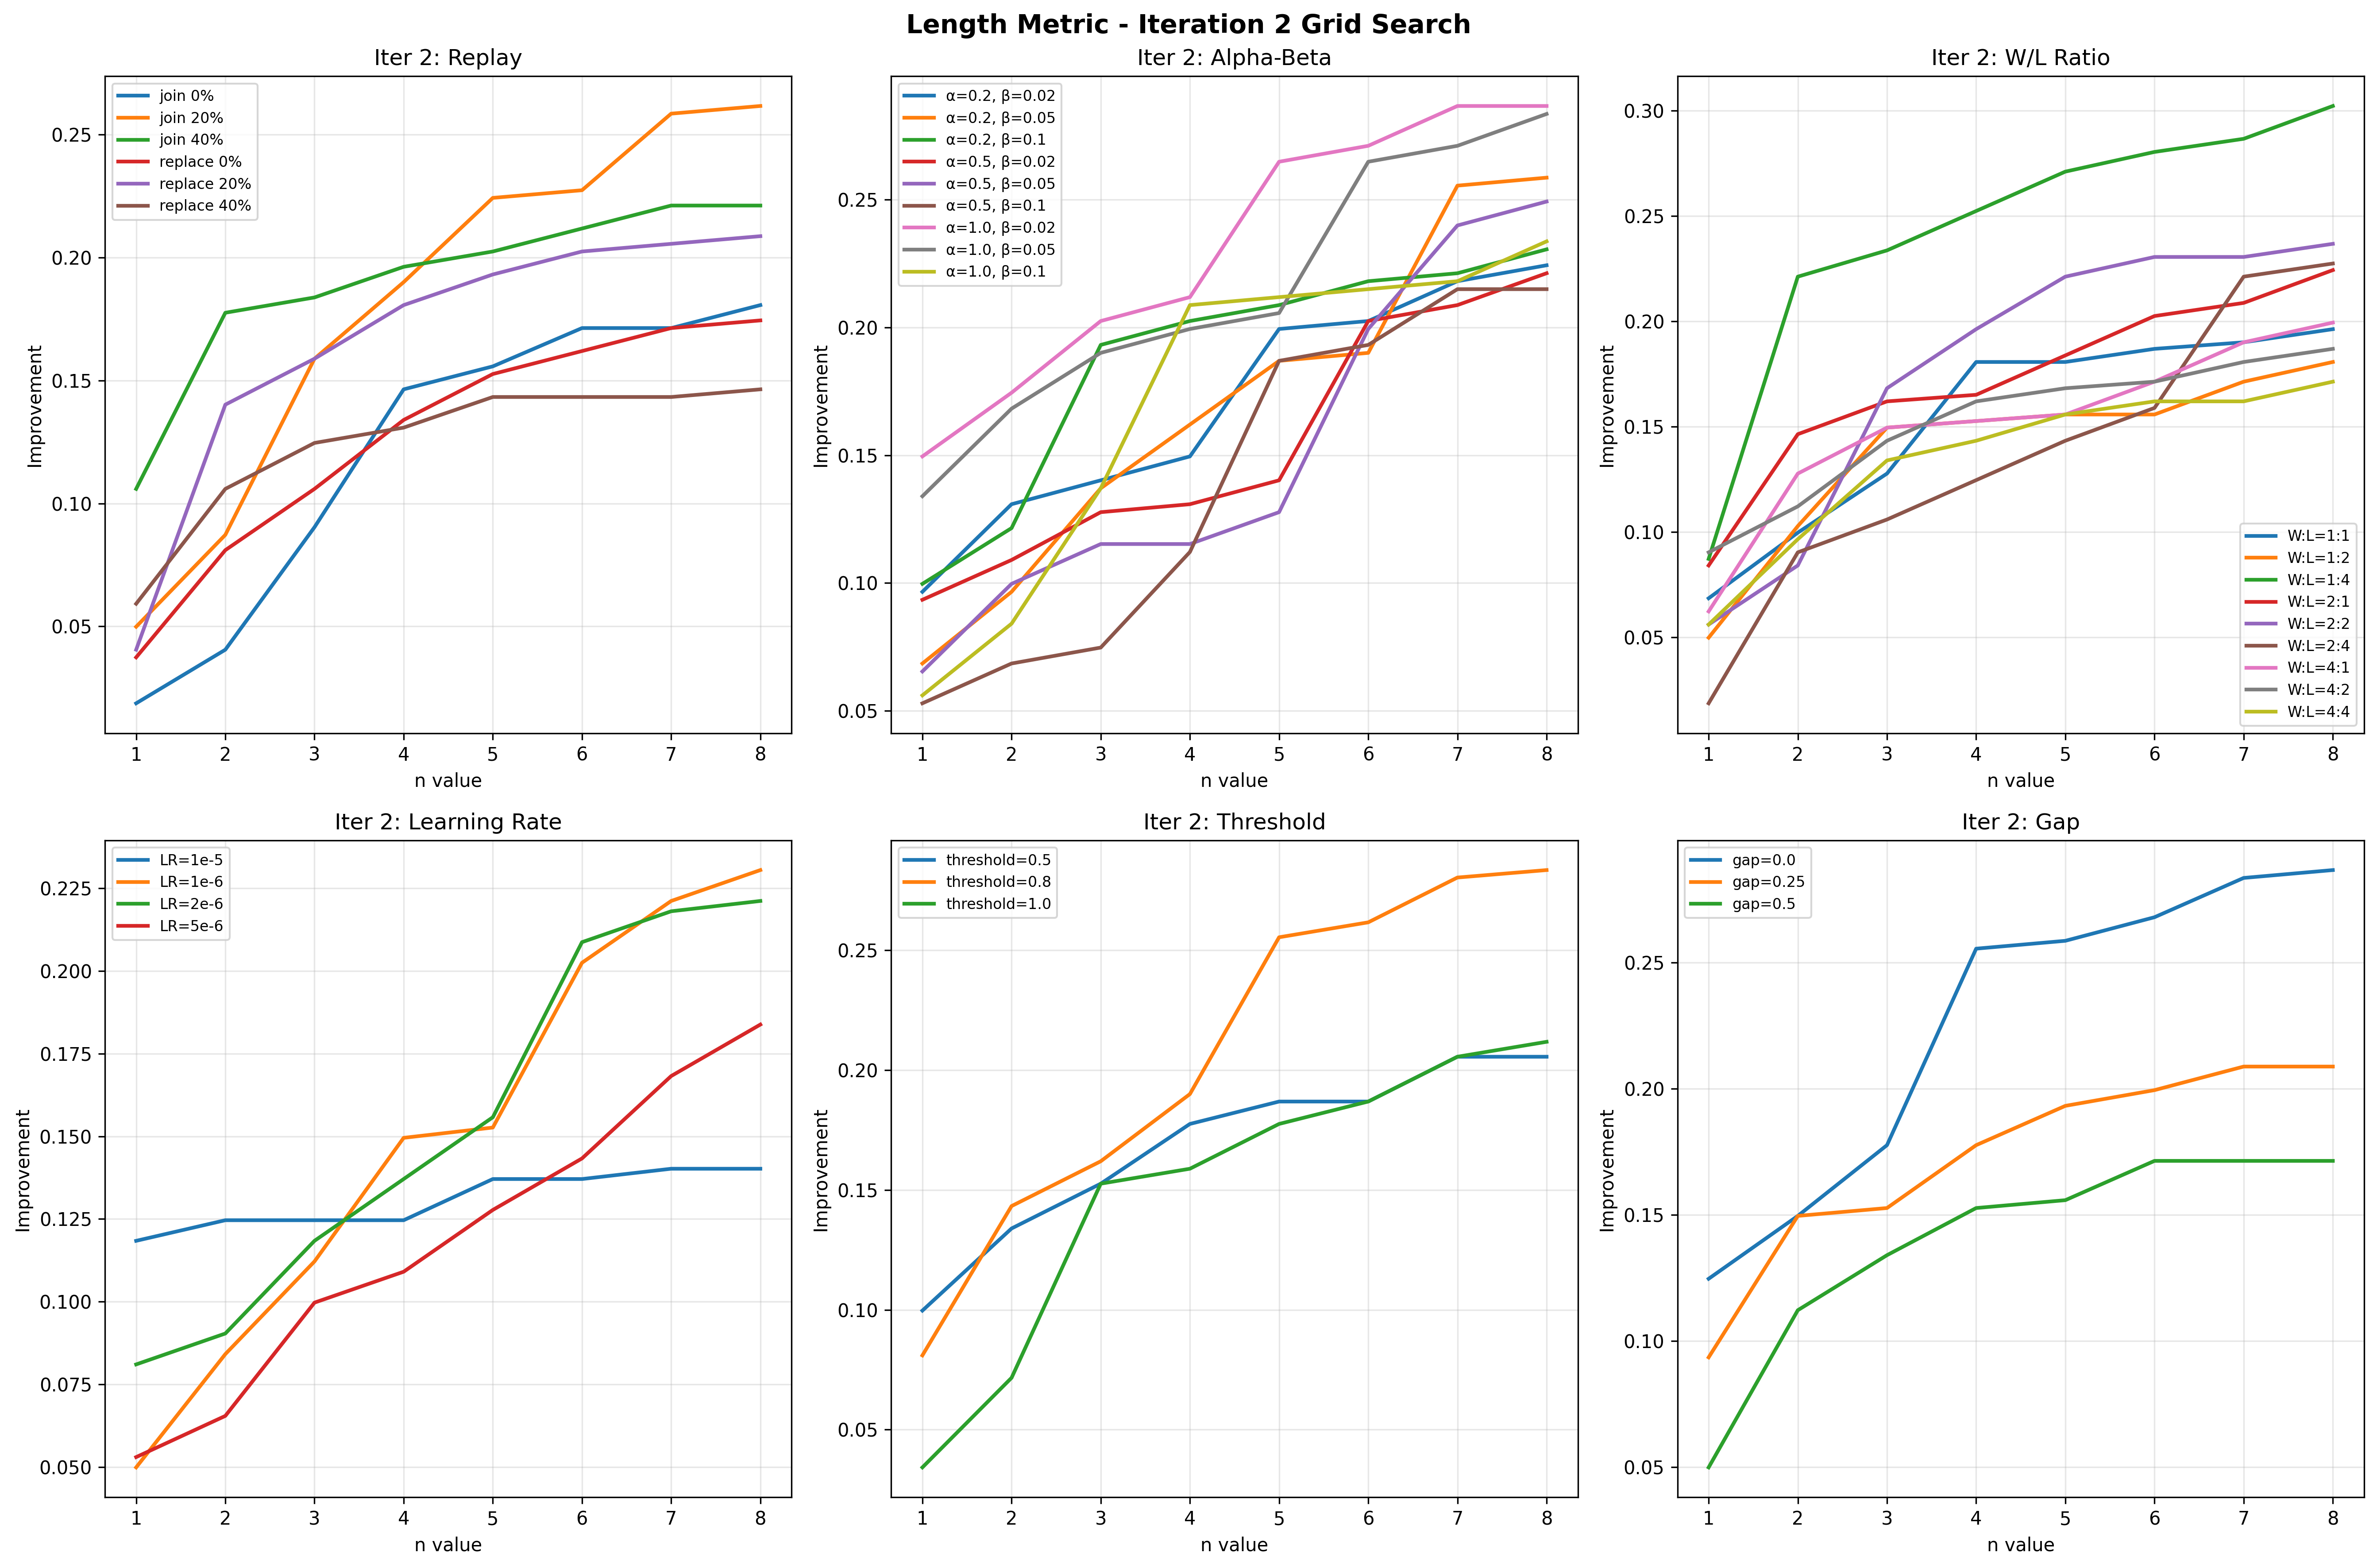
\includegraphics[width=0.65\linewidth]{figures/Length/length_iter_2_gridsearch_all.png}
  % \caption{Iteration 2.}
\end{minipage}

% \vspace{-6pt}

\begin{minipage}[t]{\linewidth}
  \centering
  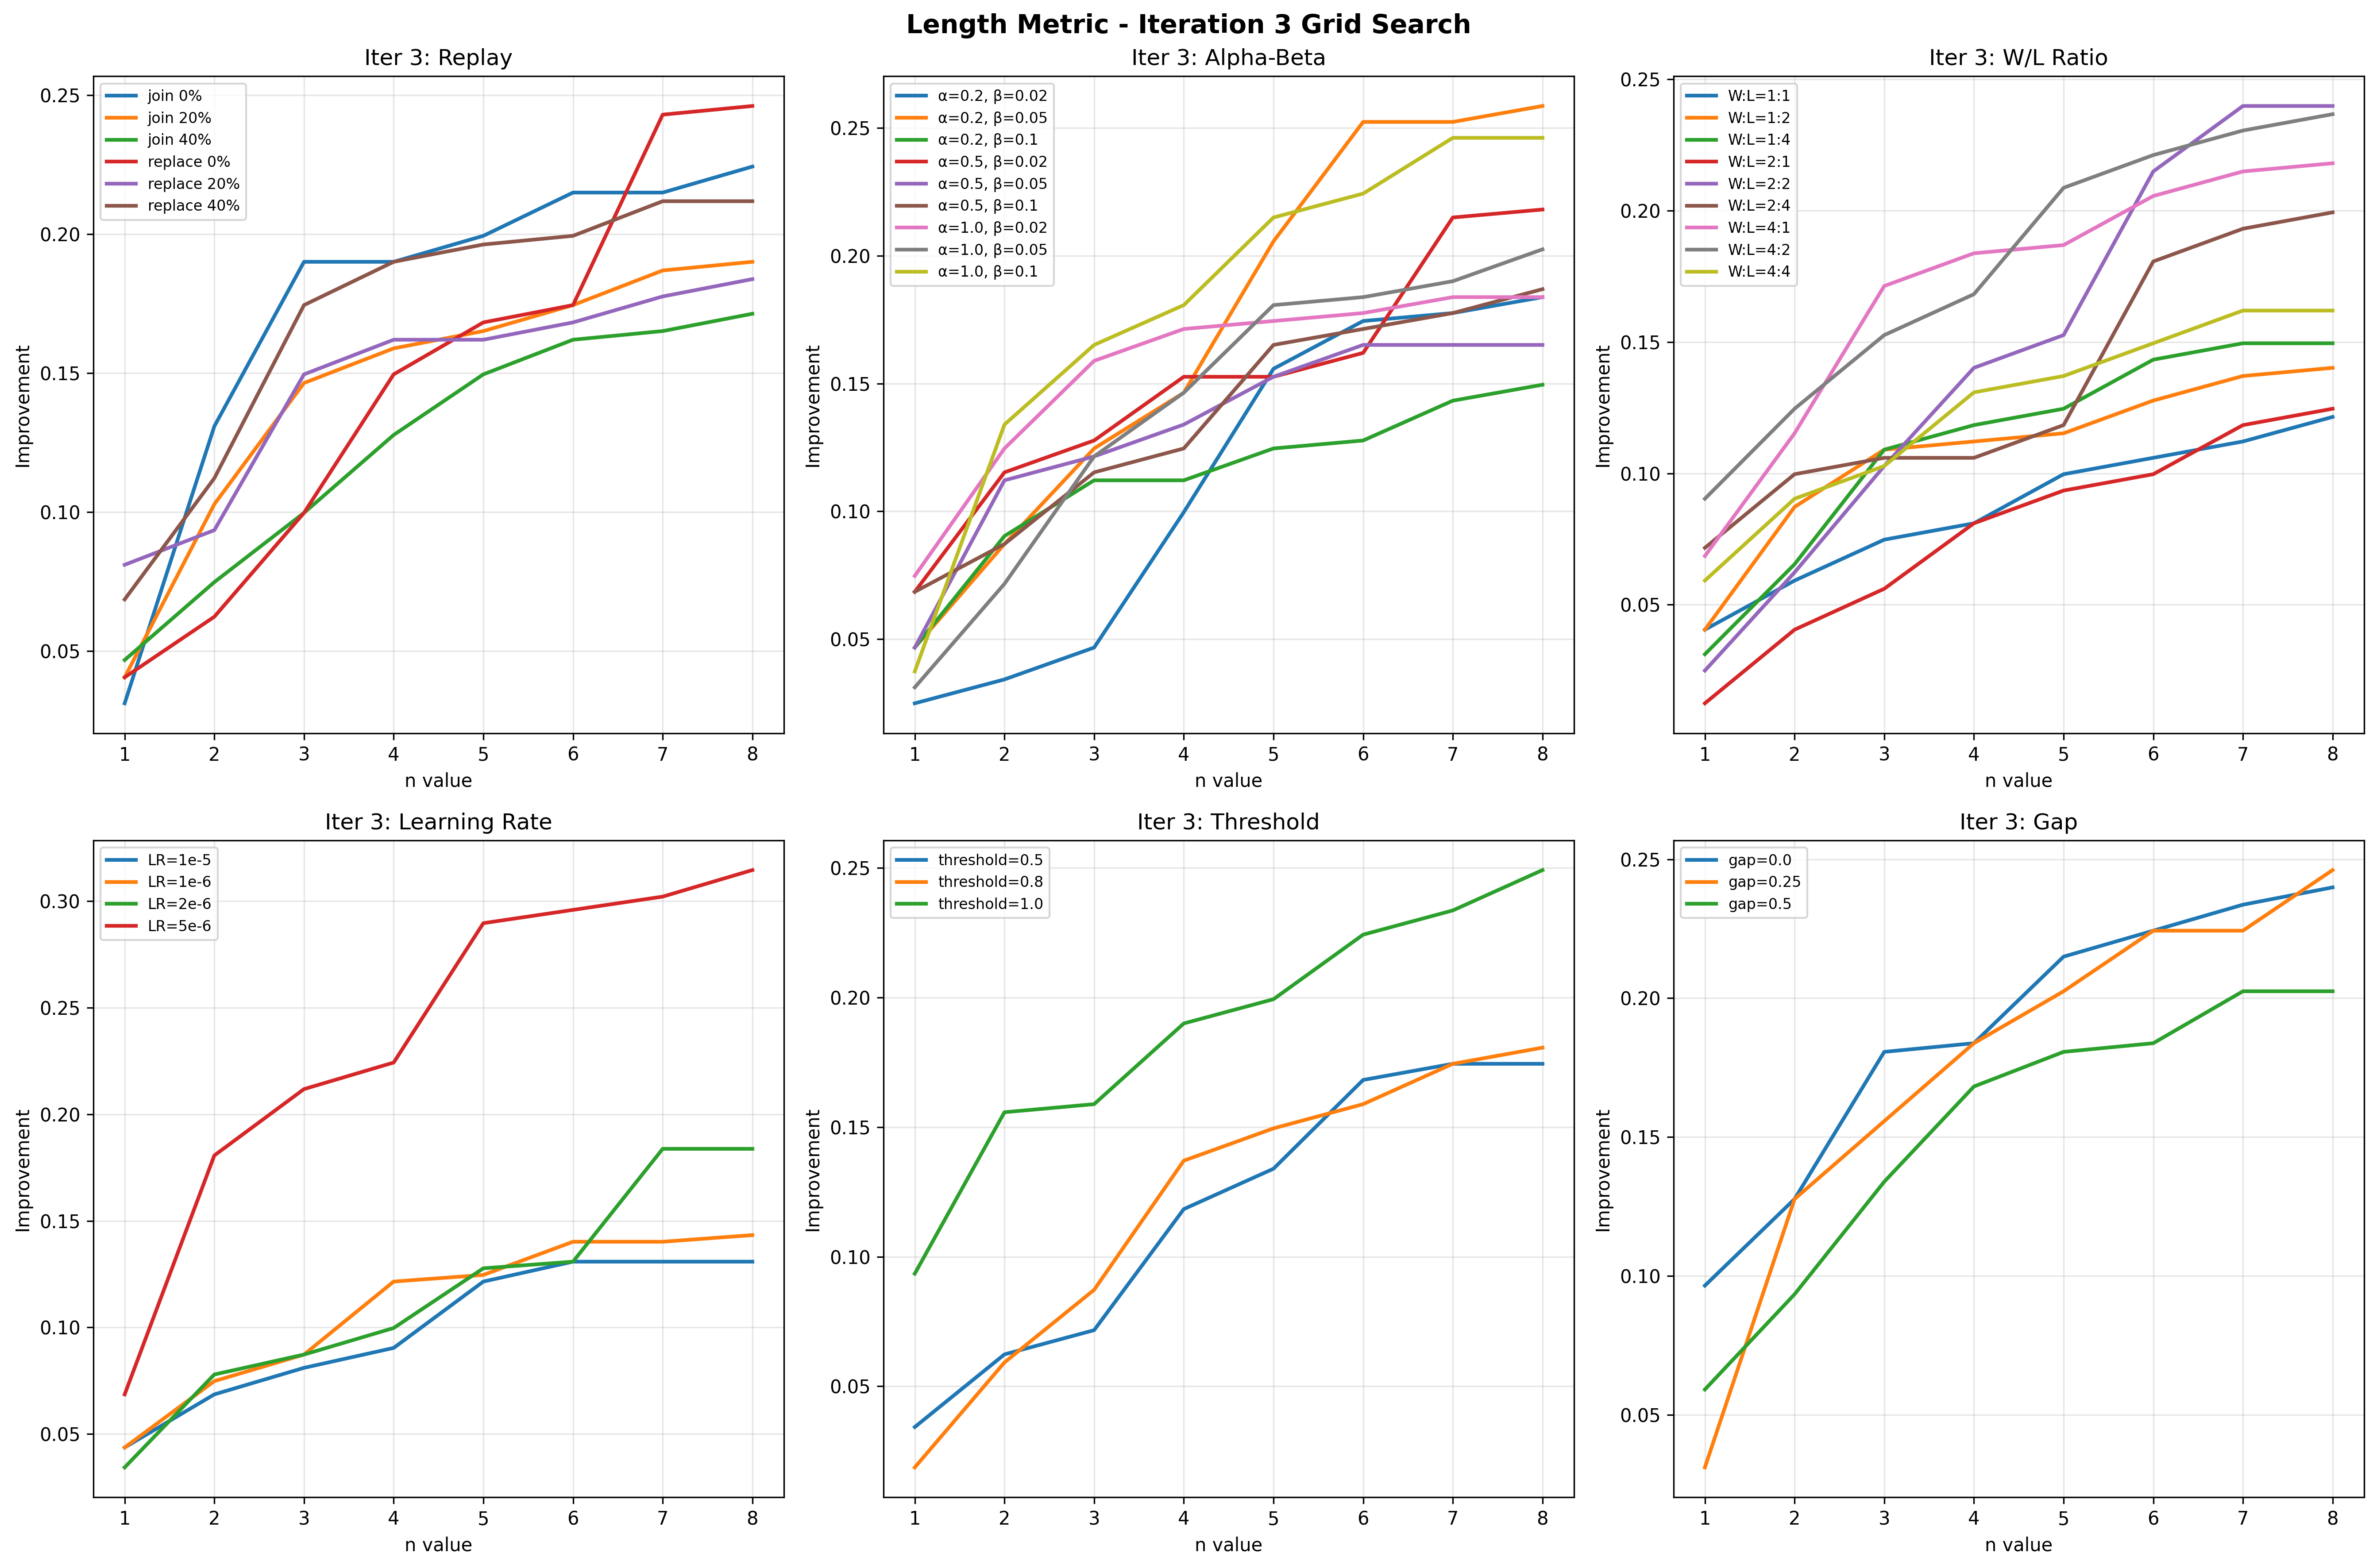
\includegraphics[width=0.65\linewidth]{figures/Length/length_iter_3_gridsearch_all.png}
  % \caption{Iteration 3.}
\end{minipage}

\caption{Hyperparameter grid searches for the \textbf{length} metric across iterations 1--3.}
\label{fig:grid_len_all}
\end{figure}
\FloatBarrier
\newpage

\begin{figure}[t]
\centering
\captionsetup{skip=4pt}

\begin{minipage}[t]{\linewidth}
  \centering
  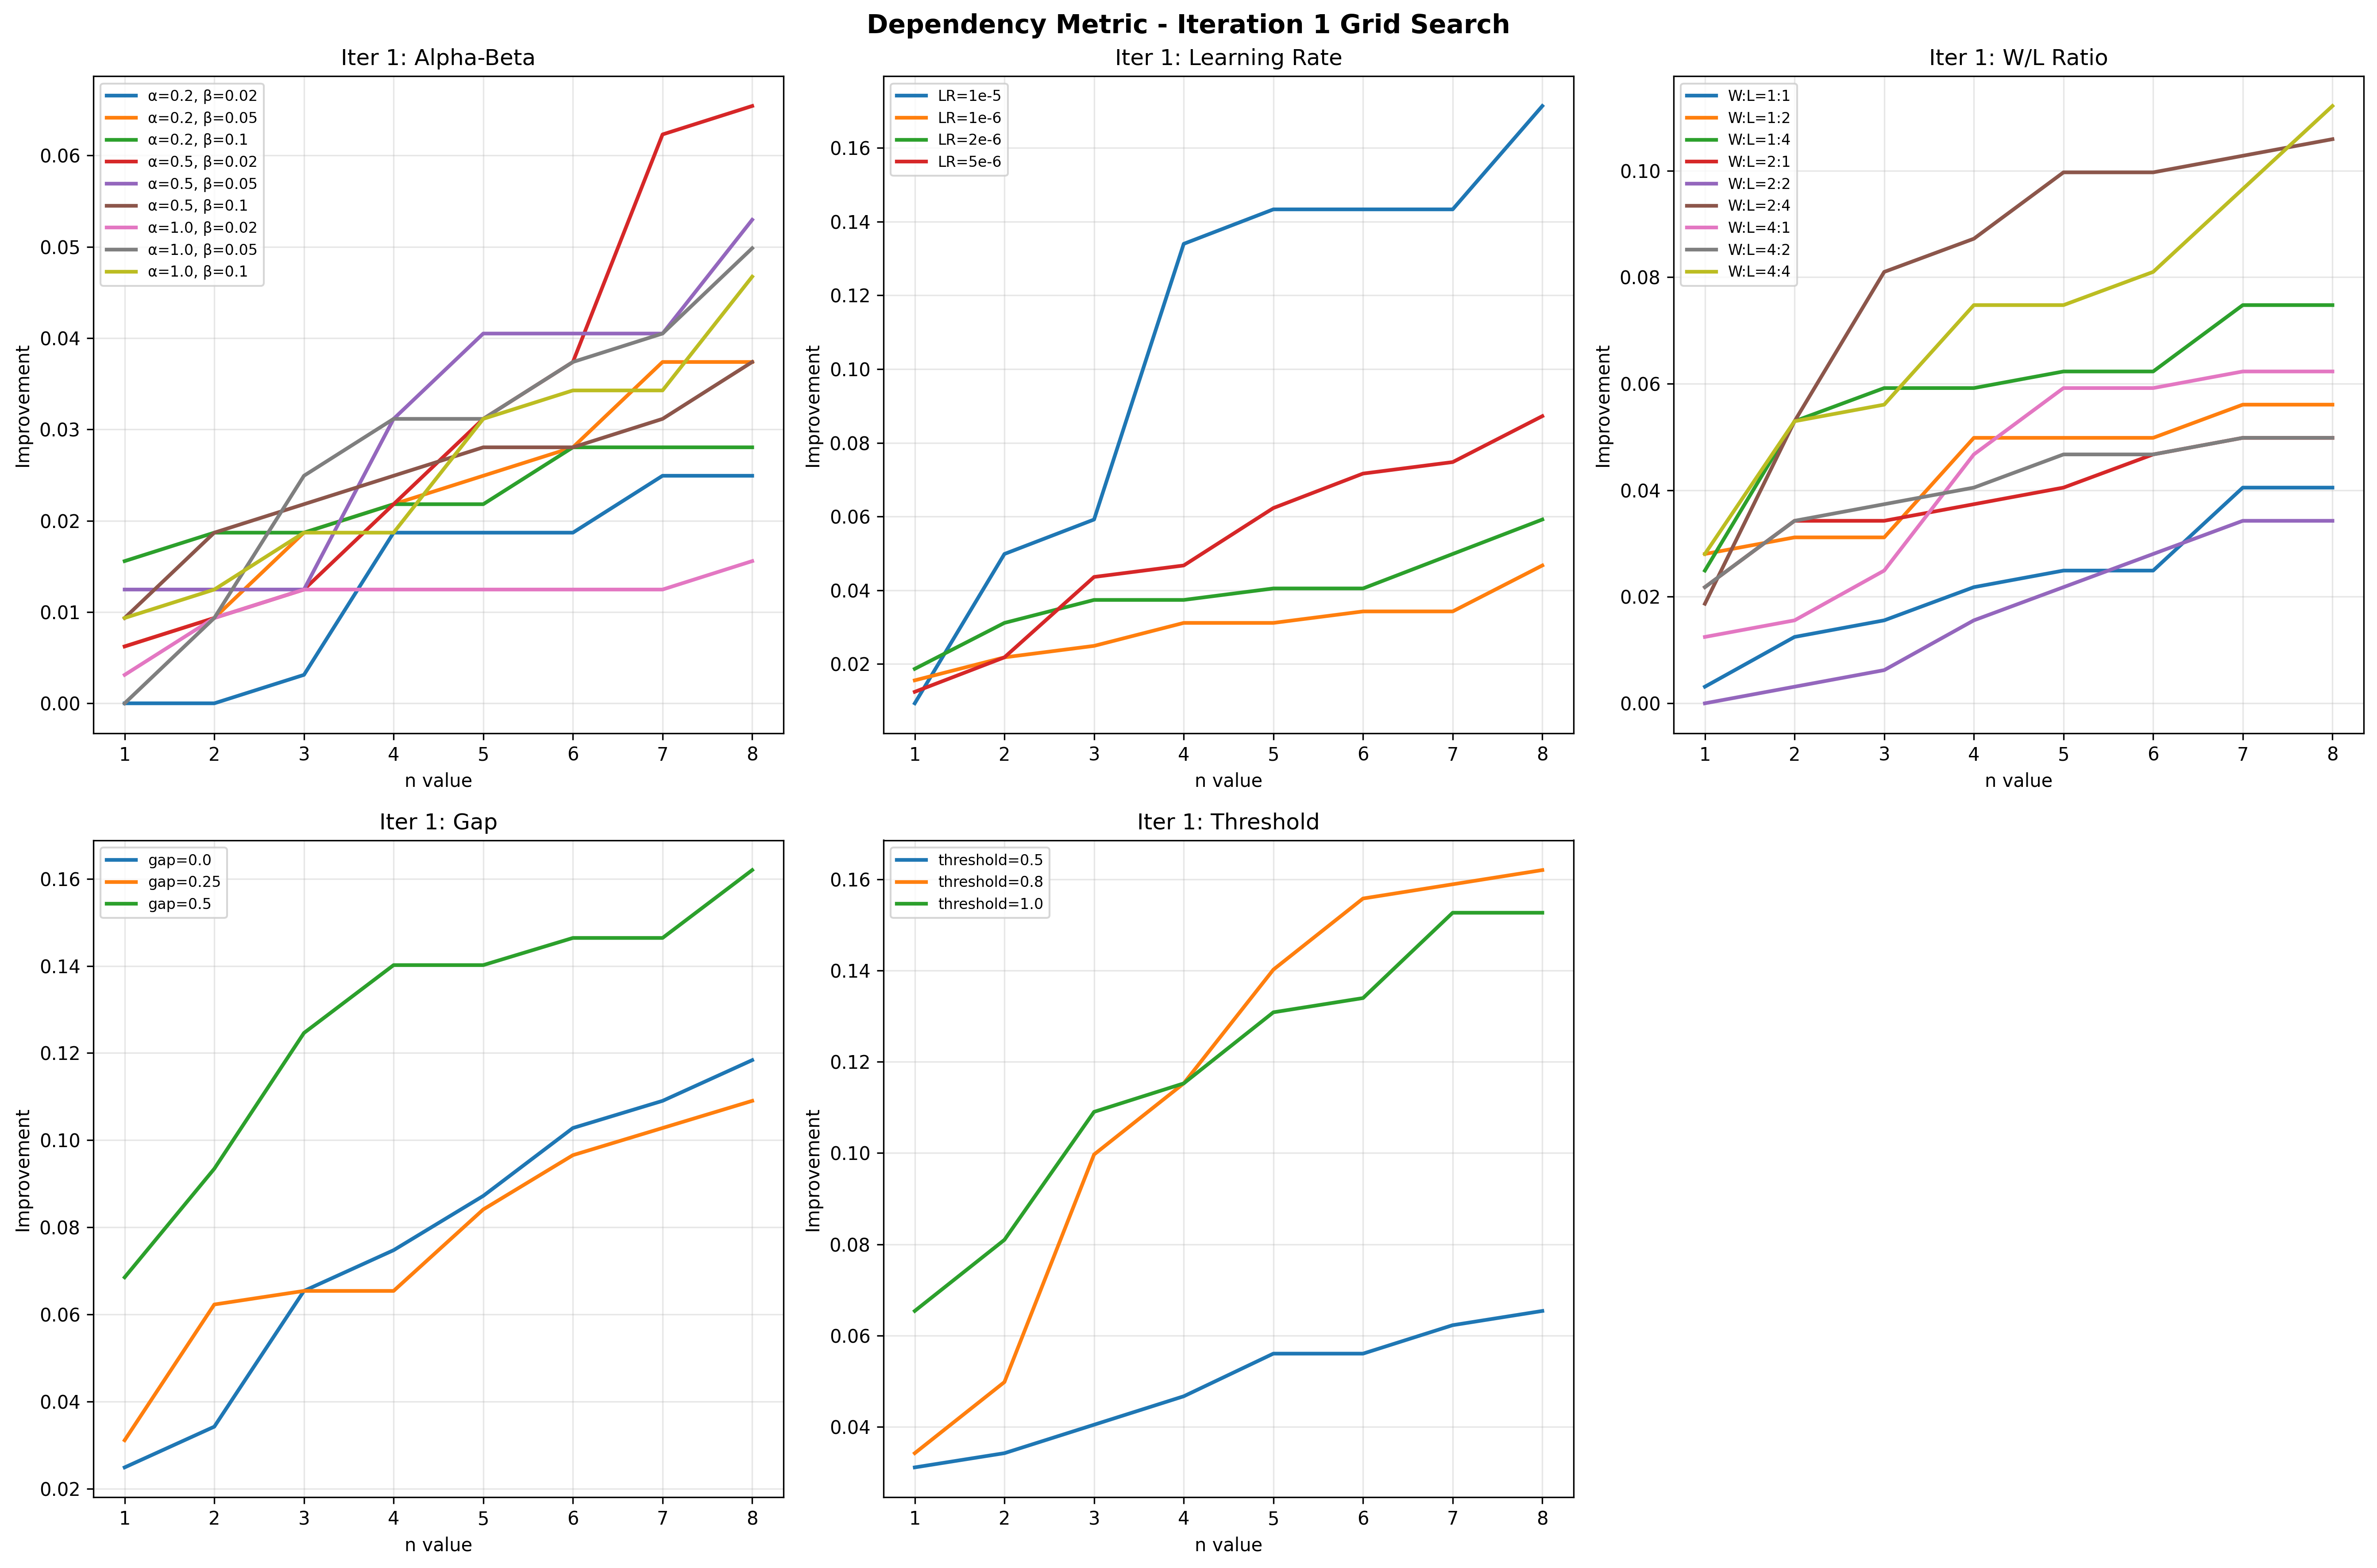
\includegraphics[width=0.65\linewidth]{figures/Dependency/dependency_iter_1_gridsearch_all.png}
  % \caption{Iteration 1.}
\end{minipage}

% \vspace{-6pt}

\begin{minipage}[t]{\linewidth}
  \centering
  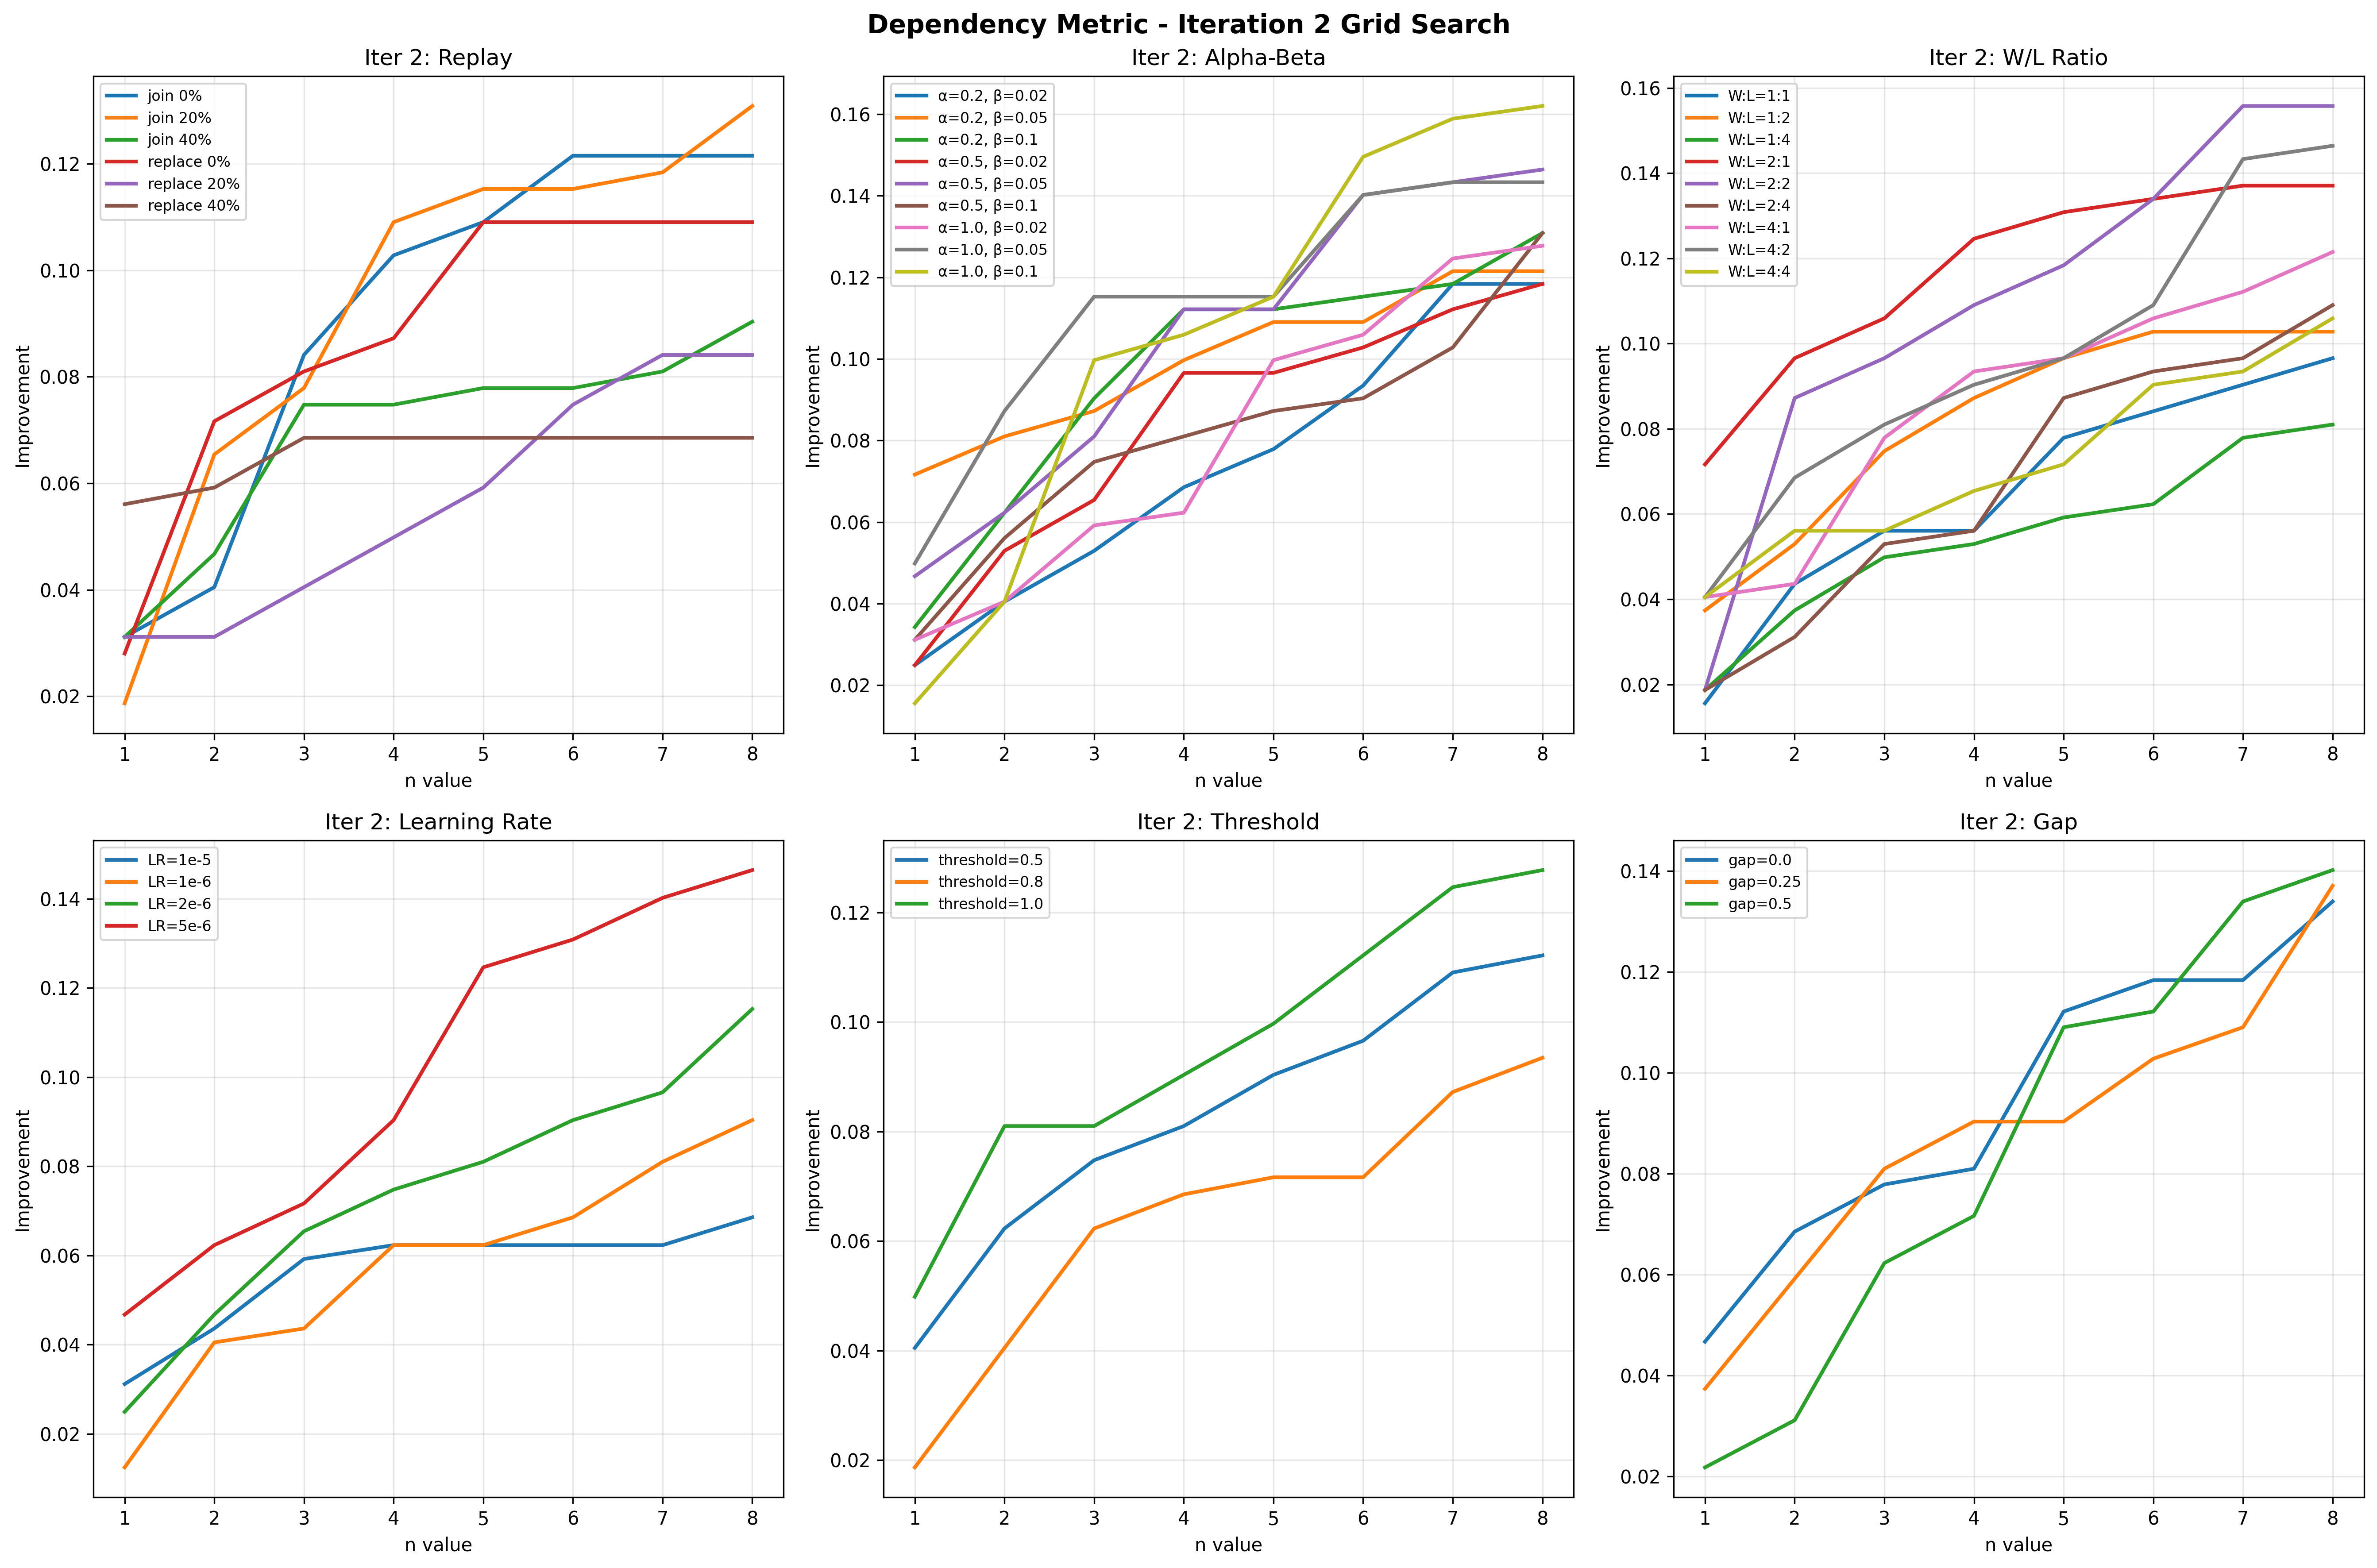
\includegraphics[width=0.65\linewidth]{figures/Dependency/dependency_iter_2_gridsearch_all.png}
  % \caption{Iteration 2.}
\end{minipage}

% \vspace{-6pt}

\begin{minipage}[t]{\linewidth}
  \centering
  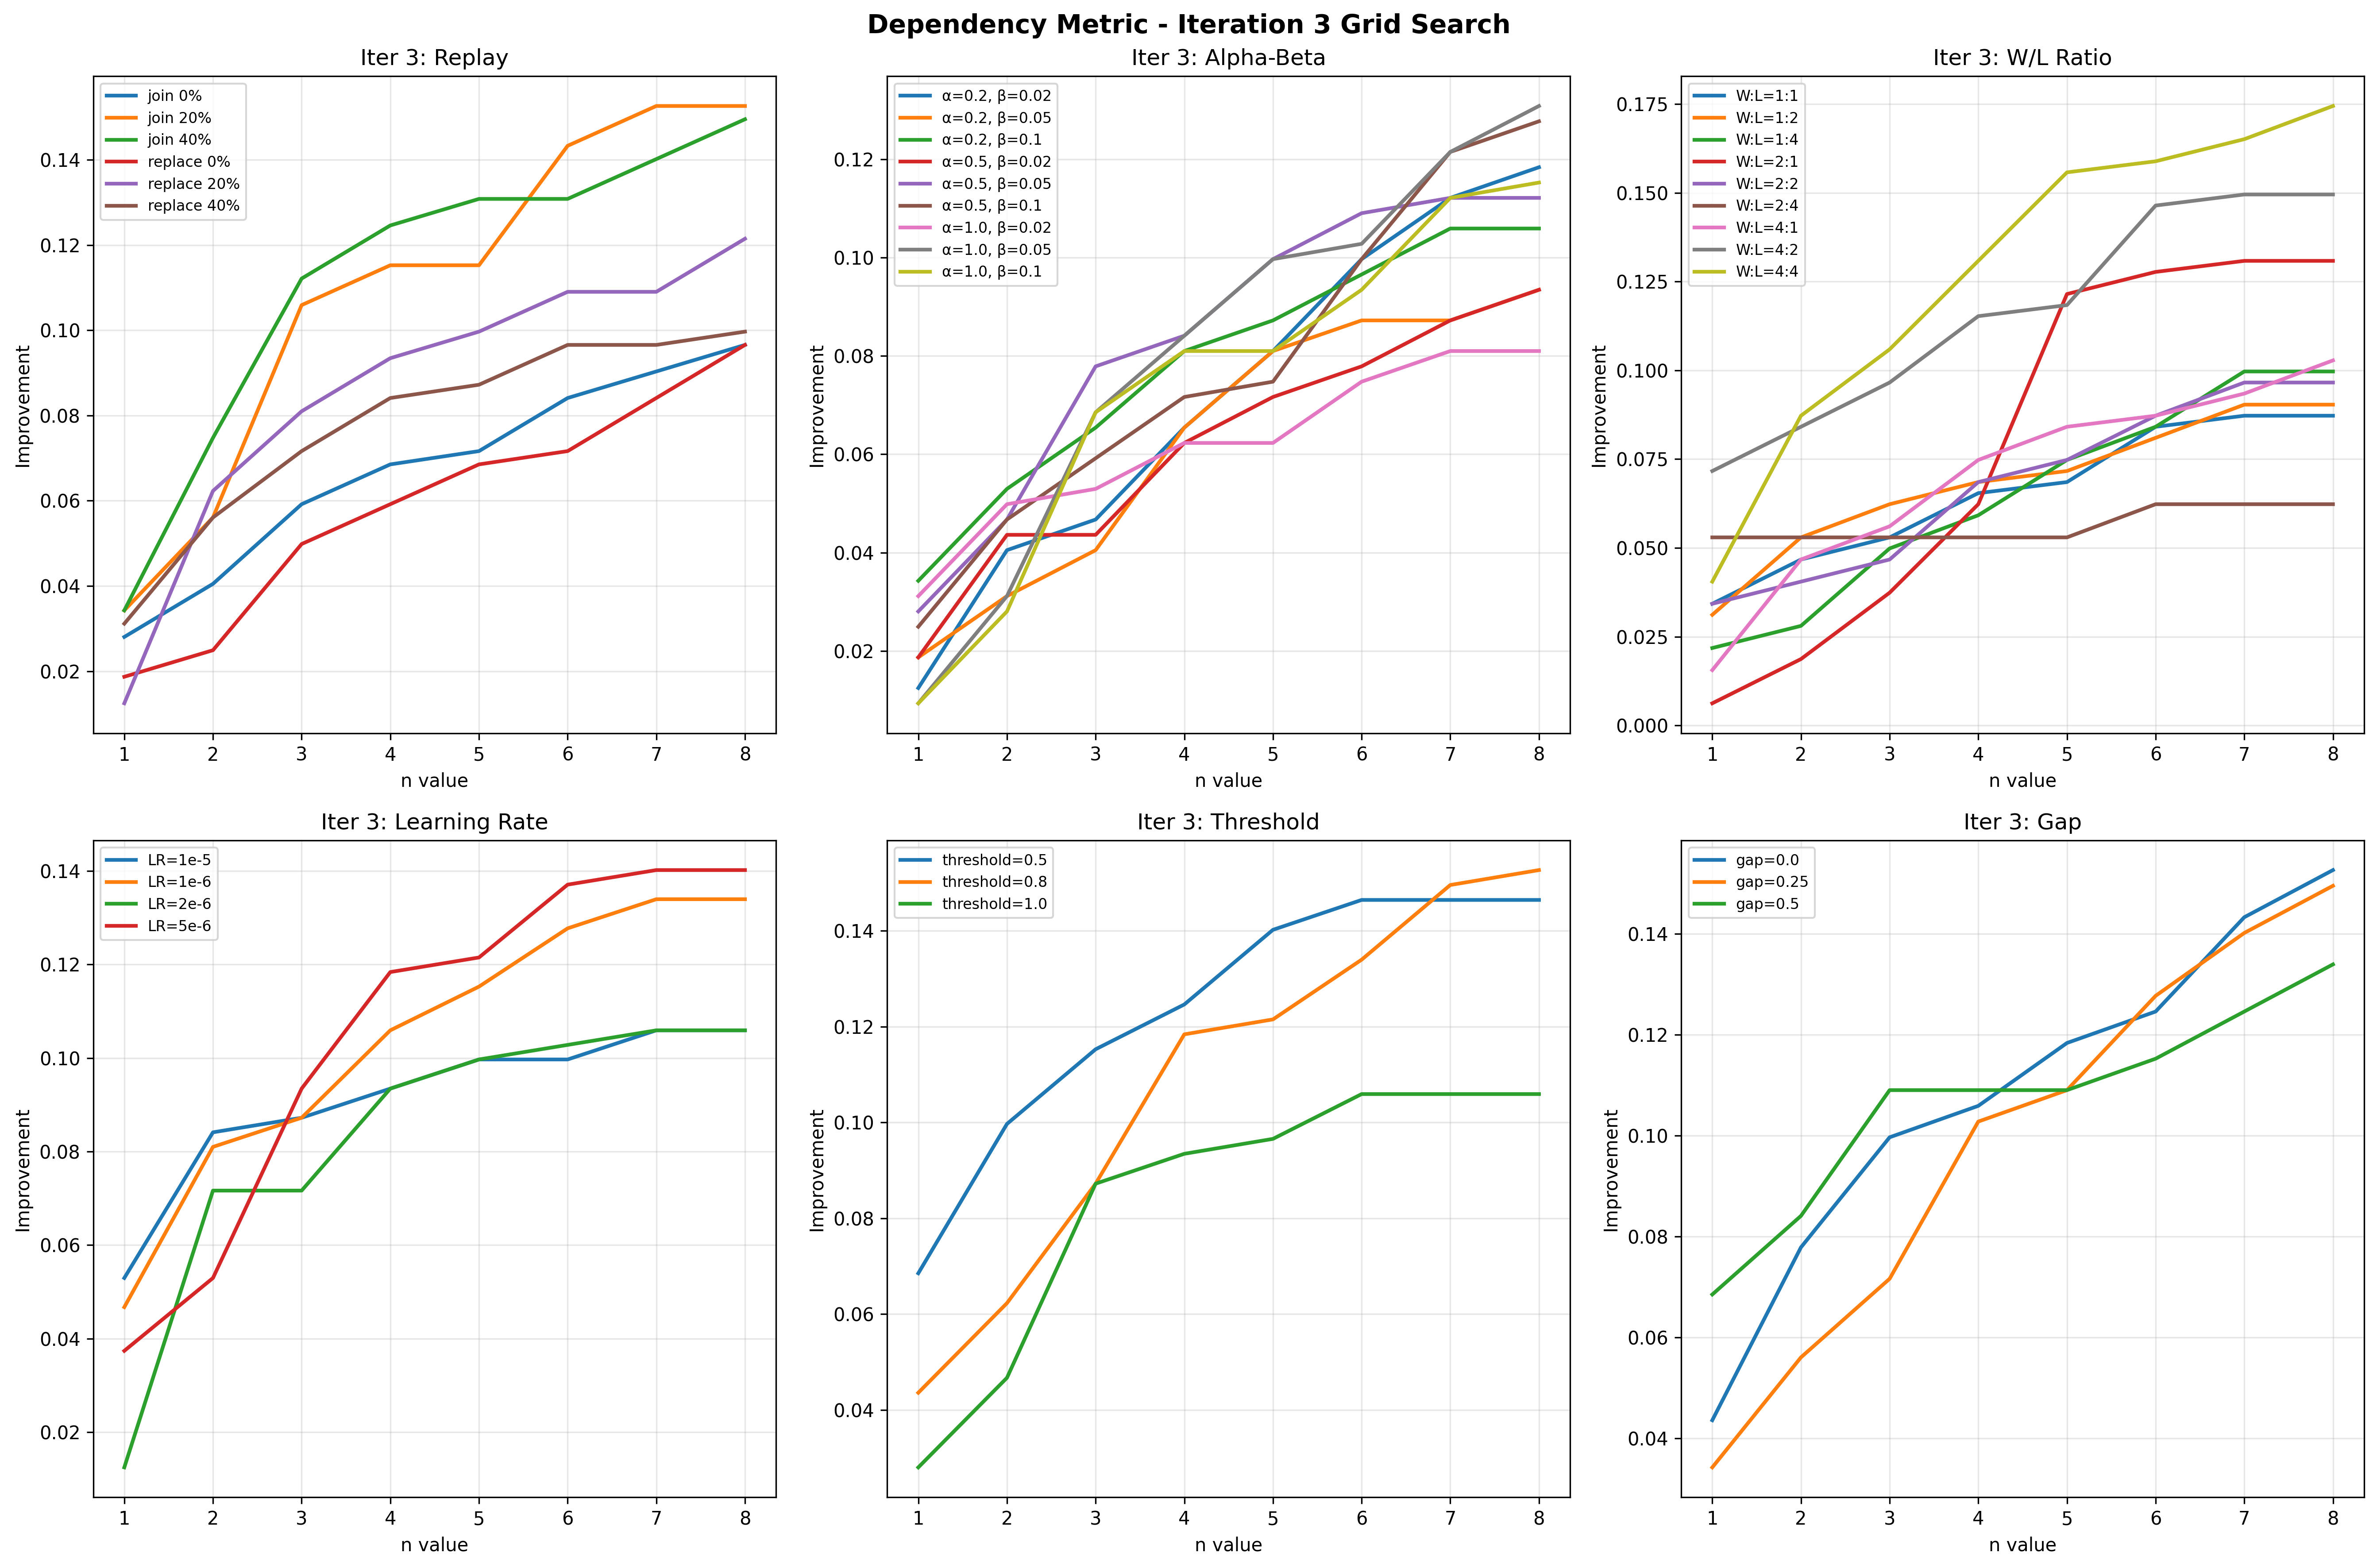
\includegraphics[width=0.65\linewidth]{figures/Dependency/dependency_iter_3_gridsearch_all.png}
  % \caption{Iteration 3.}
\end{minipage}

\caption{Hyperparameter grid searches for the \textbf{dependency} metric across iterations 1--3.}
\label{fig:grid_dep_all}
\end{figure}
